\section{Anschluss Diskettenlaufwerk}
Die Beiden Signale Dir und Step werden vom FPGA angesteuert. Da mit niedrigen 
Pegeln verwenden (vgl. \url{http://www.moria.de/~michael/floppy/floppy.pdf} p. 
21) können diese direkt mit den 3.3 V Pegeln des FPGA angesteuert werden. Mit 
Drive Select kann das Laufwerk aktiviert werden. Dazu muss das Signal nach 
Masse gezogen werden. Dazu genügt es, einen Jumper am entsprechenden Pin Nach 
Masse zu stecken. Die restlichen Pins des Floppy Bus können unbeschaltet 
bleiben. 
\begin{table}[h!]
    \centering
    \begin{zebratabular}{lll}
        \rowcolor{gray} Spartan 3E Starter Kit & $\to$ & Diskettenlaufwerk \\
        IO9 (D7)  & $\to$ & step (20) \\
        IO10 (C7) & $\to$ & dir (18) \\
    \end{zebratabular}
    \caption{Verbindung Sparten 3E Starter Kit $\to$ Diskettenlaufwerk}
    \label{tab:connection}
\end{table}
\begin{figure}[h!]
    \centering
    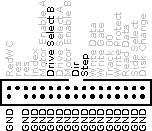
\includegraphics[width=0.3\textwidth]{../organization/floppy_connect.pdf}
    \caption{Pinbelegung Diskettenlaufwerk}
    \label{fig:pin_floppy}
\end{figure}
